\chapter{Data model}
\label{sec:data-model}

Very many difficulties users have with font editing (both scripted and
interactive) come from an incomplete understanding of the data model
involved: what entities exist in a font and a font editor and what
relationships those entities have with each other.  The distinction between
glyphs and characters seems to be an especially frequent cause of confusion. 
This chapter attempts to describe FontAnvil's data model in a way that will
be useful to script programmers.

\section{Fonts in memory}

Because PE script was originally designed for controlling a GUI font
editor, it treats fonts as documents to be opened and closed, much as
a GUI editor might.

At any given time there exists a global set of fonts that are \emph{open}. 
These are stored in RAM.  Open fonts are associated with filenames, even if
the filenames do not actually exist on disk; the interpreter will assign
temporary filenames (usually similar to ``\texttt{Untitled1.sfd}'') to fonts
that were created in memory and not loaded from files.  The filenames should
be unique (no more than one open font sharing a filename), and it's not easy
to create a situation where they are non-unique, but I suspect that having
distinct open fonts with duplicate filenames may be technically possible and
likely to trigger bugs if attempted.

The set of open fonts is technically a sequence (with a specific order), not
an unordered set, and the order is visible to scripts through the
\verb|$firstfont| and \verb|$nextfont| built-in variables, but this fact is
seldom important.

At most one of the open fonts may be the \emph{current font}.  This state is
global.  Most font-editing operations implicitly apply to the current font. 
The \texttt{Open()} built-in function sets the current font, but its exact
behaviour is context-sensitive.  If the specified filename is already an
open font, then \texttt{Open()} just sets the current font to that one.  If
the specified filename is \emph{not} already an open font, then
\texttt{Open()} loads it from disk, causing it to become an open font, before
setting the current font to that one.

When the interepreter starts up, the set of open fonts is empty and there is
no current font.  In this state, any operation that implicitly refers to the
current font will fail; scripts can only use a small subset of the language
to create or open a font and make it current.  The \texttt{Close()} built-in
function removes the current font from the set of open fonts (without saving
it to disk---that must be done as a separate operation if saving is desired)
and places the interpreter back into the state of having no current font. 
Note that the existence of a no-font state is a difference between PE script
and the FontForge GUI.  The GUI insists on always having at least one open
font and always having a current font, enforcing this rule by automatically
loading fonts from earlier editing sessions, automatically creating a new
empty font if the load fails, choosing another open font to be current when
one is closed, and terminating the program when the last font is closed.

\section{Glyphs and slots}

Here are two pictures of Don Quixote.\footnote{Left: Gustave
Dor\'{e}, 1863.  Right: Honor\'{e} Daumier, 1868.}

\begin{center}

\includegraphics[width=1.5in]{quixote-dore.jpg}\qquad
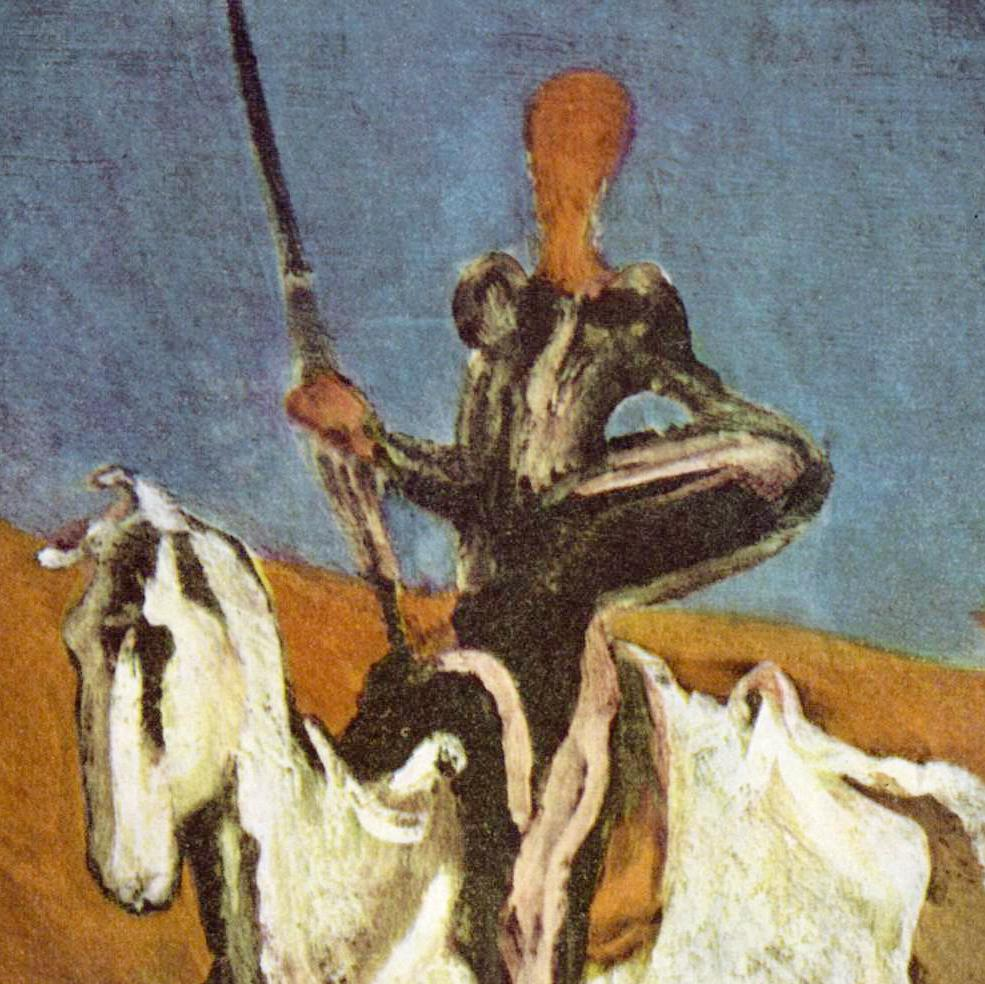
\includegraphics[width=1.5in]{quixote-daumier.jpg}
\end{center}

The pictures are different, but they are pictures of the same fictional
character.  In the same way, we can have several pictures of the same
character in a writing system.

\begin{center}
\scalebox{4}{a}\qquad
\scalebox{4}{\textit{a}}\qquad
\scalebox{4}{\texttt{a}}
\end{center}

What these three ``a''s share is the \emph{character}; what they do not
share is the \emph{glyph}.  Fonts contain collections of glyphs, concrete
things, which are pictures of characters, abstract things.  It is often the
case that in any given font, each glyph corresponds to exactly one character
and vice versa; but there are many important exceptions to that rule.  To
understand how FontAnvil processes fonts it is important to bear in mind
that fonts are collections of glyphs, and glyphs are not the same thing as
characters despite being closely connected with characters.

This glyph (the classic ff-ligature) is not associated with one character,
but with a sequence of two characters:

\begin{center}
\scalebox{5}{ff}
\end{center}

There is no double-f character, as a separate abstract entity distinct from
just two ordinary ``f''s in a row, in the English language.  There is no
standard character code for such a thing.\footnote{Actually, there is one in
Unicode, but you're not supposed to really use it; the details of that are
beyond the scope of this discussion.} Nonetheless a font for high-quality
typesetting of English must contain a glyph for this double-f entity
that is not quite a character.  Despite such exceptions, one glyph per
character is true most of the time in English.  In some other languages, the
conceit of glyph-character equivalence breaks down entirely.  In Arabic, for
example, many characters have four or more visual forms requiring
separate glyphs in a font, depending on how they connect to neighbouring
characters.

FontAnvil represents a font in memory as including a zero-based array of
\emph{glyph slots}.  The array is variable-sized, but it is a true array
data structure, not a list: all slots from index 0 up to one less than the
number of slots exist as long as the in-memory font does.  Creating a new
glyph means overwriting the possibly-blank previous contents of some slot. 
Destroying a glyph means filling the slot with a blank glyph, but the slot
continues to exist.  Changing the number of slots can only be done by
increasing or decreasing the length of the array, and encodings (described
in the next section) may constrain the number of slots.

Glyph slots in a font always have \emph{glyph numbers} which are their
indices in the array.  Glyphs in a font cannot meaningfully be said to be in
any specific order other than the order determined by the array indices. 
Every glyph has a number, and every number has a glyph slot.  No two glyphs
can have the same slot; two slots may contain identical glyphs, or even a
``reference'' from one to the other, but the two slots' contents will not
truly be the same entity.  A glyph slot might be \emph{blank}, that is
devoid of outlines and other data, and people usually think of such slots as
not really being glyphs.  But some attributes of a glyph slot (such as its
name) are required to always have non-null values, even on blank slots.

\begin{framed}
FontAnvil's in-memory glyph slots can be blank but never truly empty. 
However, most on-disk file formats \emph{do} have a concept of a glyph
failing to exist at all.  Blank slots are usually not written when saving
from memory to disk, and loading a file from disk to memory that does not
fill all slots will usually leave the others blank.
\end{framed}

Every open font has a \emph{selection}, which specifies a set of the glyph
slots (more about glyph slots in the next section).  Many editing operations
implicitly operate on the selection of the current font.  Although every
open font has a selection, usually only the selection of the current font is
relevant.  Open fonts retain their selections through changes in which open
font is current.

The selection is actually a sequence, not a set, of glyph slots.  That means
the slots in it can be selected in a specific order.  This distinction is
relevant in the FontForge GUI, where you can select several glyphs in a
specific order, open a ``Metrics'' window, and have them come up in the
order you selected them.  However, each glyph slot can appear at most once
in the selection, and the order of the selection is seldom if ever
observable or controllable from the scripting language.  It is usually
better to think of it as a set with no specific order, not as a sequence.

The selection is applied at the level of glyph slots.  It is perfectly
possible for the selection to include blank glyph slots, because it is
defined as a set of slots, not a set of non-blank glyphs.  Nonetheless, one
often only cares about the non-blank glyphs, and some commands for
manipulating the selection will automatically limit themselves to slots that
are not blank.

Glyph slot numbers \emph{may or may not} be closely connected to Unicode,
ASCII, or other character codes, depending on issues discussed in the next
section.  It is important to be aware that glyph slot numbers are not the
same type of entity as character codes, despite sometimes having equal
numerical values.

\section{Encodings}

Fonts do not exist solely to be edited with FontAnvil.  To be useful, a font
must eventually be saved in some format understandable by a word processor
or similar application; and the external software must be able to associate
the glyphs in the font with the characters in text that will be typeset
using the font.  There will necessarily exist some \emph{code} that
associates numbers called \emph{code points} with the different characters
that might appear in text, and a font file must explicitly or implicitly
describe which code points go with which glyphs.  It is worth emphasizing
that code points refer to characters, \emph{not glyphs}.

The ASCII code is familiar to many computer users, especially in the
English-speaking world, but is inadequate for languages other than English. 
Today, nearly everybody uses a code called Unicode.  Unicode's code points
coincide with ASCII for all the characters covered by ASCII; but it also
covers many thousands of other characters.  It is supposed to be a universal
code for all text in all human languages.  But Unicode did not always exist and its use was not always
universal.  Most common font formats are designed to also accomodate
character encoding schemes predating Unicode or simply other than Unicode. 
Frequently, a font file will include translation mappings for several
different codes, in the hope that software using the font can find its own
preferred code among the choices.  There needs to be a way to translate code
points (which identify characters) into glyph numbers (which identify
glyphs), even in cases like ligatures and variant glyphs where this
translation is more complicated than a simple one-to-one lookup.

FontAnvil includes several mechanisms for addressing these issues, but the
most significant is that of the \emph{encoding}.  The encoding is a
property of each font (global to the font) and describes a set of
assumptions and constraints about the relationships between code points and
glyph numbers.

\begin{framed}
Every glyph slot in a font always has a glyph number, no two slots can have
the same number, and the set of glyph numbers that exist is always the set
of integers from 0 up to one less than the number of glyphs in the font. 
Every code point designates at most one glyph slot.  But a glyph slot might
have zero, one, or more than one code point; a code point might have no
glyph slot; and the set of code points that exist might not be a simple
interval of the integers.  Nonetheless, the font's encoding may trigger the
enforcement of constraints that make the code point situation less
complicated.
\end{framed}

Most of the possible values of the encoding field are associated with
standardized character codes defined by external organizations.  Each code
defines a meaning for a range of code points from 0 up to some number that
depends on the code.  \emph{When the encoding is associated with an
externally standardized code other than Unicode}, FontAnvil enforces the
following constraints:
\begin{itemize}
\item There must be at least as many glyph slots as there are code points in
the code.
\item Glyph slots in the range 0 through one less than the number of code
points in the code correspond one-to-one with the code points.
\item Any glyph slots with greater indices have no code points.
\end{itemize}

The case of \emph{unencoded glyphs}, those in glyph slots beyond the end of
the code point range specified by the encoding, is important.  Glyphs like
the ff-ligature mentioned earlier, or the alternate forms of letters in a
script like Arabic, usually fall into this category.  When a word processor
typesets text using a font, it starts out by translating the code points
into glyphs one-for-one according to the basic code points of the glyph. 
The result of that translation cannot contain unencoded glyphs.  But the
basic one-for-one translation of code points to glyphs is only a starting
point.  Further processes can merge and split glyphs so that more than one
character can be typeset with one glyph, one character can be typeset with
more than one glyph, and which glyph goes with which character can be
different in different contexts.  These further processes can bring
unencoded glyphs into play.  The encoding does not specify the number of
unencoded glyph slots that may exist after the range of encoded glyphs.  The
unencoded glyph slots may be manipulated by built-in functions like
\texttt{SetCharCnt()}; encoded glyph slots may not be added or removed.

Each glyph slot has a property called the \emph{Unicode number}.  This is a
code point (in the code that is named Unicode), but I am going to call the
number in this field just a ``number'' to distinguish it from the code
points that exist in non-Unicode encodings.  When the encoding is one of the
standardized non-Unicode encodings, the constraint is enforced that the
Unicode number must be the correct translation (using the iconv library) of
the glyph number for encoded glyphs, or the null value of -1 for unencoded
glyphs.  For example, if the font's encoding is KOI8-R (commonly used for
Russian text), then glyph slot number 241 is for the letter ``ya,'' which
looks like a backwards R.  FontAnvil will enforce the constraint that this
slot's Unicode number is 0x042F, which is the Unicode code point for that
letter.  ``The constraint is enforced'' means that if you try to change the
value of the Unicode number field, the font's encoding will be immediately
changed to Custom.  Editing the Unicode numbers is not compatible with
keeping the encoding and its fixed mapping.

But not every value for the font's global encoding field is associated with
an external standard other than Unicode.  When the font's encoding field
refers to some form of Unicode, or does not refer to an external standard,
then additional special considerations apply; and in fact, these special
cases are the most popular and useful values for the encoding field.

When the encoding is set to Custom, few encoding-related constraints are
enforced.  There may be any number of glyph slots.  Any slot may have a
Unicode number, or not, and there is not necessarily any relationship
between the Unicode numbers and the glyph slots.

There are two Unicode encoding options, Unicode (BMP) and Unicode (Full). 
These each behave more or less like the non-Unicode standardized encodings. 
One difference is that it appears sometimes possible to set the Unicode
number of a glyph slot such that it does not match its glyph number.  This
may be a bug.  FIXME investigate further - this description may possibly be
simplified if Unicode and non-Unicode turn out to really behave the same.

FIXME investigate and document the ``Original'' encoding option.

Glyph slots have names.  All glyph slots have non-empty names, including
blank slots, and all names must be unique within a font.  The names are
sometimes automatically assigned and may also be manipulated by script
commands; but constraints (including the requirement for uniqueness) will be
enforced on such manipulation.

\begin{framed}
People who think they want to edit glyph slot names are often wrong.
\end{framed}

FIXME document name lists

\section{The \texttt{.notdef} glyph}

FIXME

\section{The clipboard}

There is a global entity called the \emph{clipboard}, which holds glyph data
of the kind that might be stored in glyph slots, such as outlines, anchors,
and references.  The clipboard is like a font in that it can store a bunch
of slots' worth of data, in a definite order, but the clipboard is unlike a
font in that the slots do not have meaningful numbers and it does not store
slot attributes other than glyph data, such as slot names and code points. 

The usual way of using the clipboard is somewhat like using the clipboard in
any common GUI document editor: select some slots, do a cut or copy
operation, select some other slots (even in a different font), and do a
paste operation.  Here is typical code to copy the uppercase ASCII alphabet
from an existing font into a new font (leaving many things in the new font
empty or default, which may cause problems later):

\begin{verbatim}
Open("font1.sfd");
Select('A','Z');
Copy();
New();
Select('A','Z');
Paste();
Save("font2.sfd");
\end{verbatim}

One thing to be aware of is that \texttt{Paste()} always writes into the
selection, and so you must create a nonempty selection for \texttt{Paste()}
to be meaningful.  This differs from a word processor that can ``insert''
text; FontAnvil treats a font as fixed framework of glyph slots that can
only be changed by overwriting.  Inserting or deleting in the middle, in a
way that changes the number of slots that exist, would disrupt the framework
of the encoding and is rarely, if ever, what you really want.

\begin{framed}
A glyph slot's name is associated with the glyph slot, not with the glyph
data stored in the slot.  The slot name will not move with the glyph data
when the glyph data is cut and pasted into a new slot.  Unicode code points,
and any other encoding numbers, are also parts of the glyph slot and will
not move with cut and pasted glyph data.
\end{framed}

\section{Look-up tables}

FIXME

